\section{Programmbeschreibung}
\label{sec:programmbeschreibung}

% Allgemeine Programmbeschreibung
\subsection{Allgemeiner Programmablauf}
\label{ssec:allgemeiner_programmablauf}

% Beschreibung der Klassen und Schnittstellen
Wie bereits in der Verfahrensbeschreibung beschrieben, werden folgende Datenstrukturen (insbesondere Klassen) benötigt:
\begin{itemize}
    \item Eine Klasse \texttt{Controller} zum Steuern der Spidercam, siehe \ref{sssec:controller}.
    \item Eine Klasse \texttt{Spidercam} zum Modellieren der Spidercam, siehe \ref{sssec:spidercam}.
    \item Eine Klasse \texttt{Movement} zum Modellieren der Bewegungen der Spidercam, siehe \ref{sssec:movement}.
    \item Eine Klasse \texttt{Phase} zum Modellieren der Phasen der Bewegungen der Spidercam, siehe \ref{sssec:phase}.
\end{itemize}

Die Klassen stehen wie in Abbildung \ref{fig:classes} dargestellt in Beziehung zueinander.

Zum Start des Programms wird die Datei \texttt{\_\_main\_\_.py} ausgeführt.
Diese Datei enthält die Hauptfunktion des Programms.
Sie ließt eine Konfigurationsdatei \texttt{config.ini} und Argumente aus der Kommandozeile ein und überprüft diese auf Korrektheit.

Anschließend wird für alle definierten Eingabedateien ein \texttt{Controller}-Objekt instanziiert.
Dieses Objekt aktualisiert bzw. instruiert die Spidercam dann zu den entsprechenden diskreten Zeitpunkten.
Zu jedem Zeitpunkt wird die Position der Spidercam bestimmt und die Längen zu den Verankerungspunkten der Drahtseile berechnet.
Die Simulation stoppt dann, wenn der \texttt{Controller} keine weiteren Instruktionen mehr hat und die Spidercam alle Bewegungen ausgeführt hat.

Anschließend werden die Ergebnisse entsprechend in die Ausgabedateien geschrieben.

% Beschreibung der Aufrufhierarchie
Die Aufrufhierarchie ist beispielhaft in Abbildung \ref{fig:sequence} zu sehen.

\begin{figure}[H]
    \centering
    % rotate=90 and span whole page
    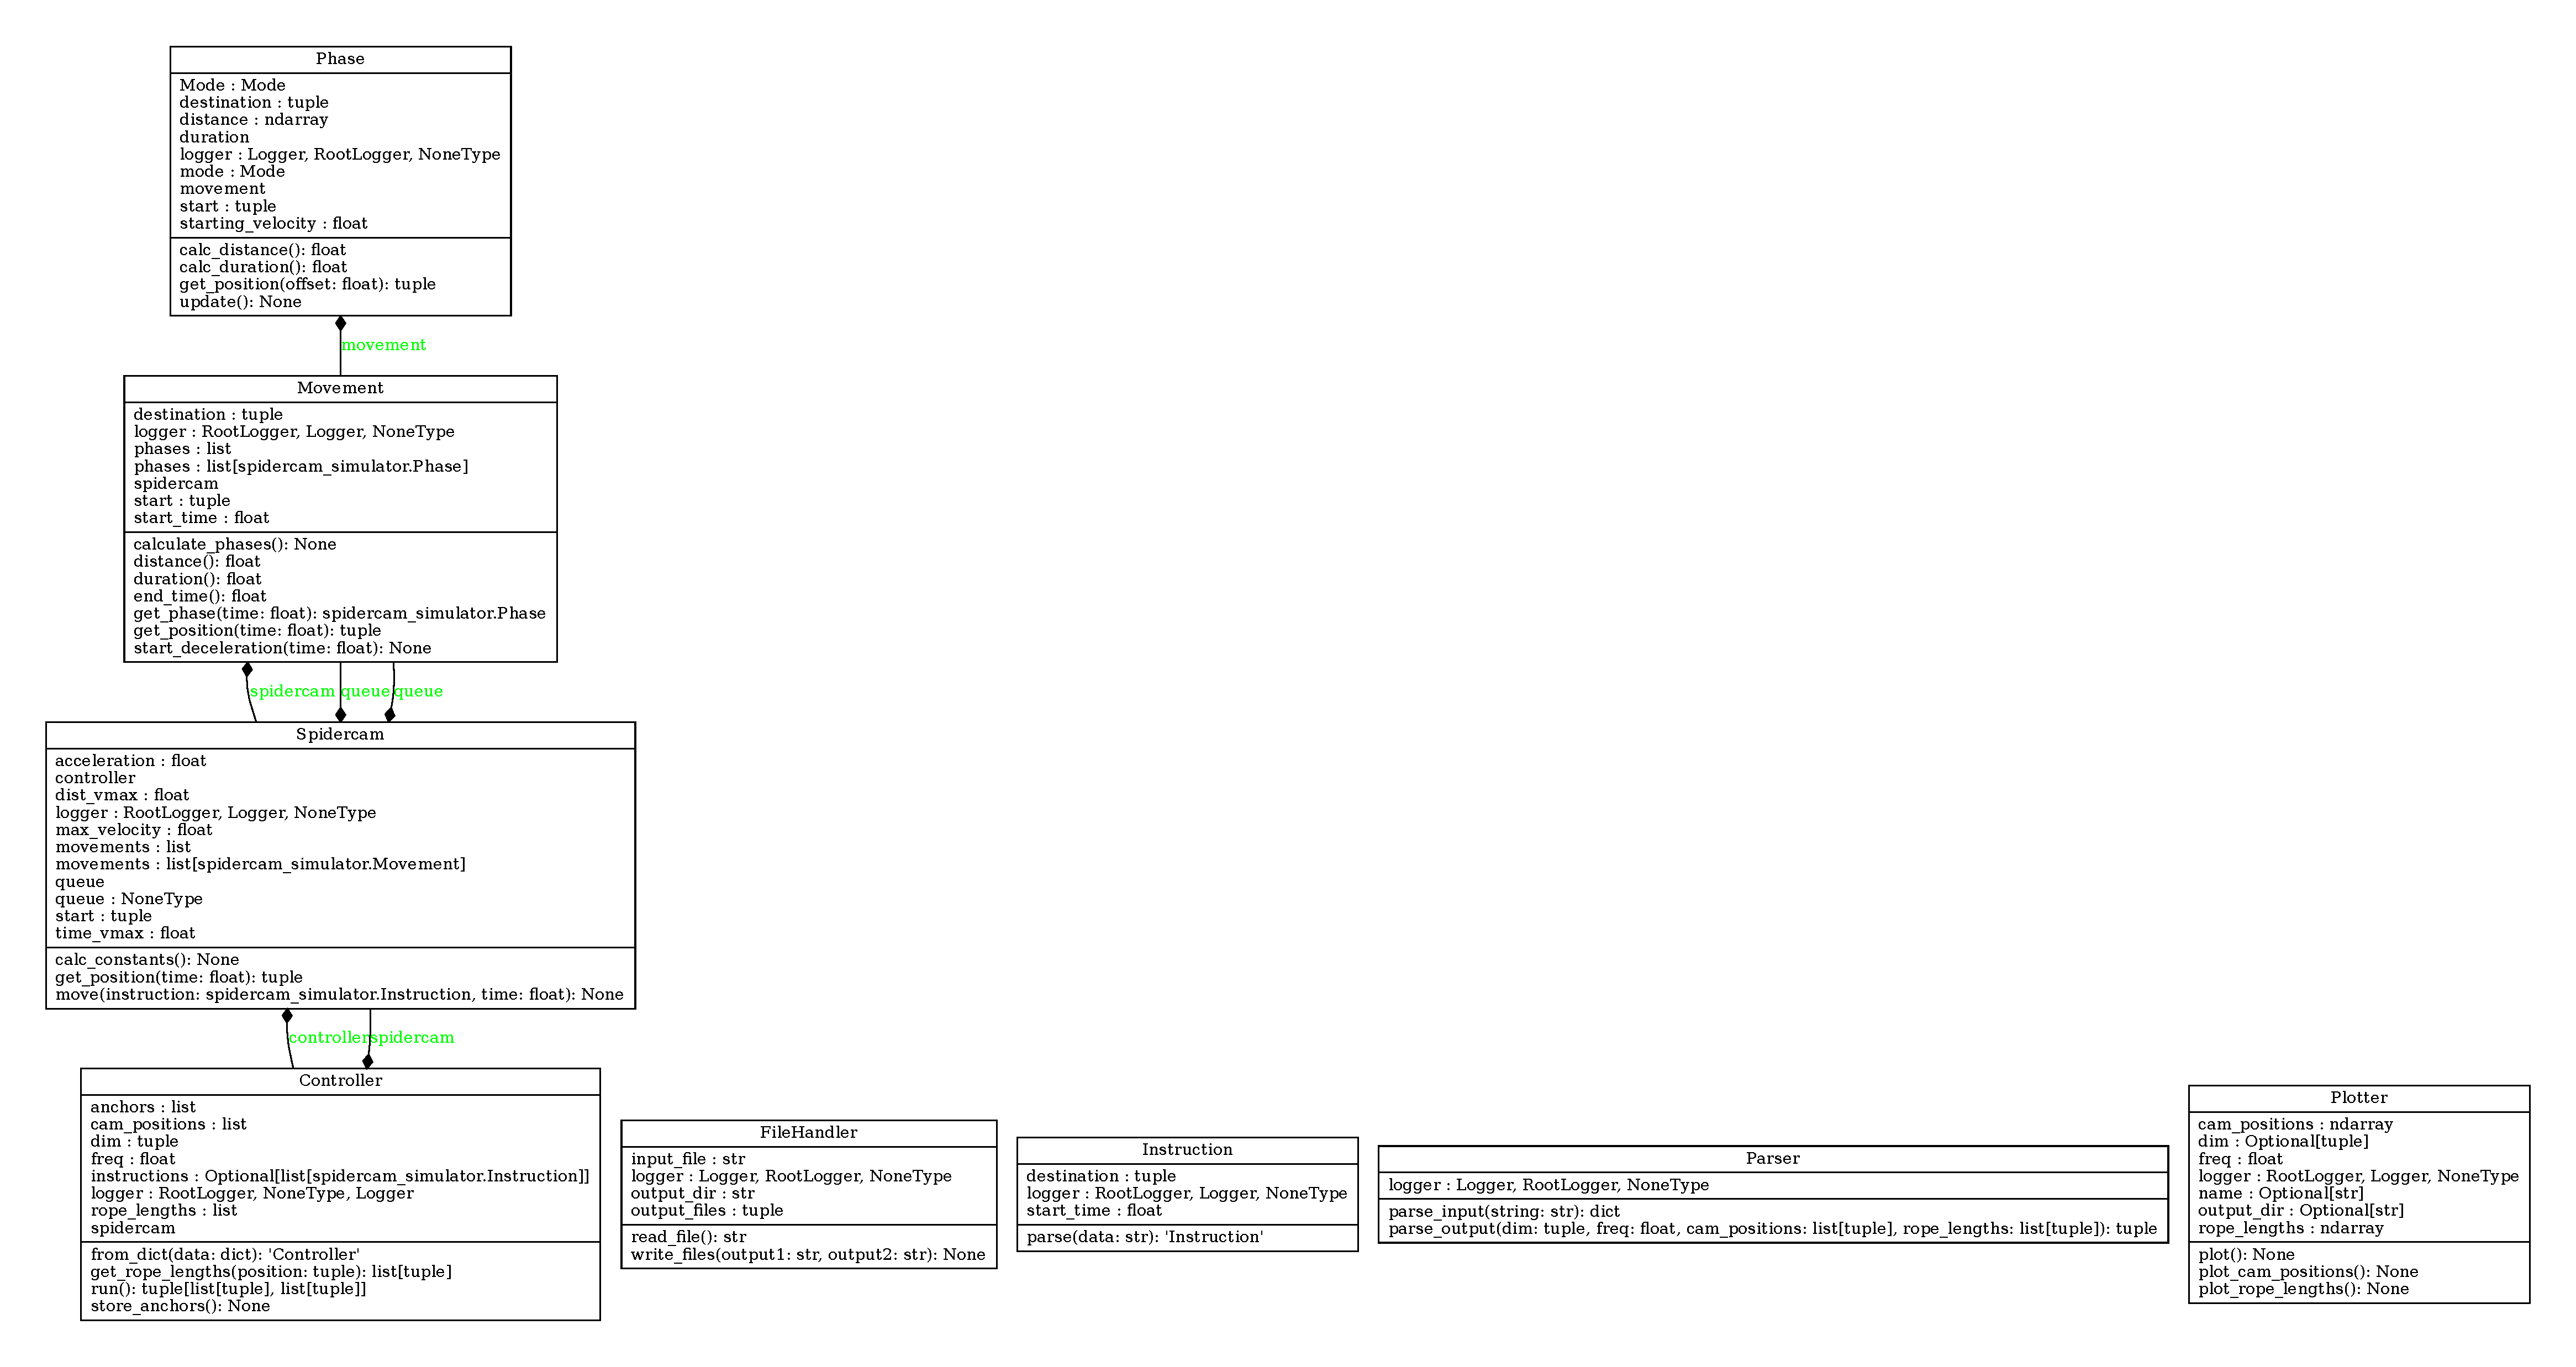
\includegraphics[width=.7\textwidth]{../python/uml/classes.pdf}
    \caption{Klassendiagramm des Programms}
    \label{fig:classes}
\end{figure}

\begin{figure}[H]
    \centering
    % rotate=90 and span whole page
    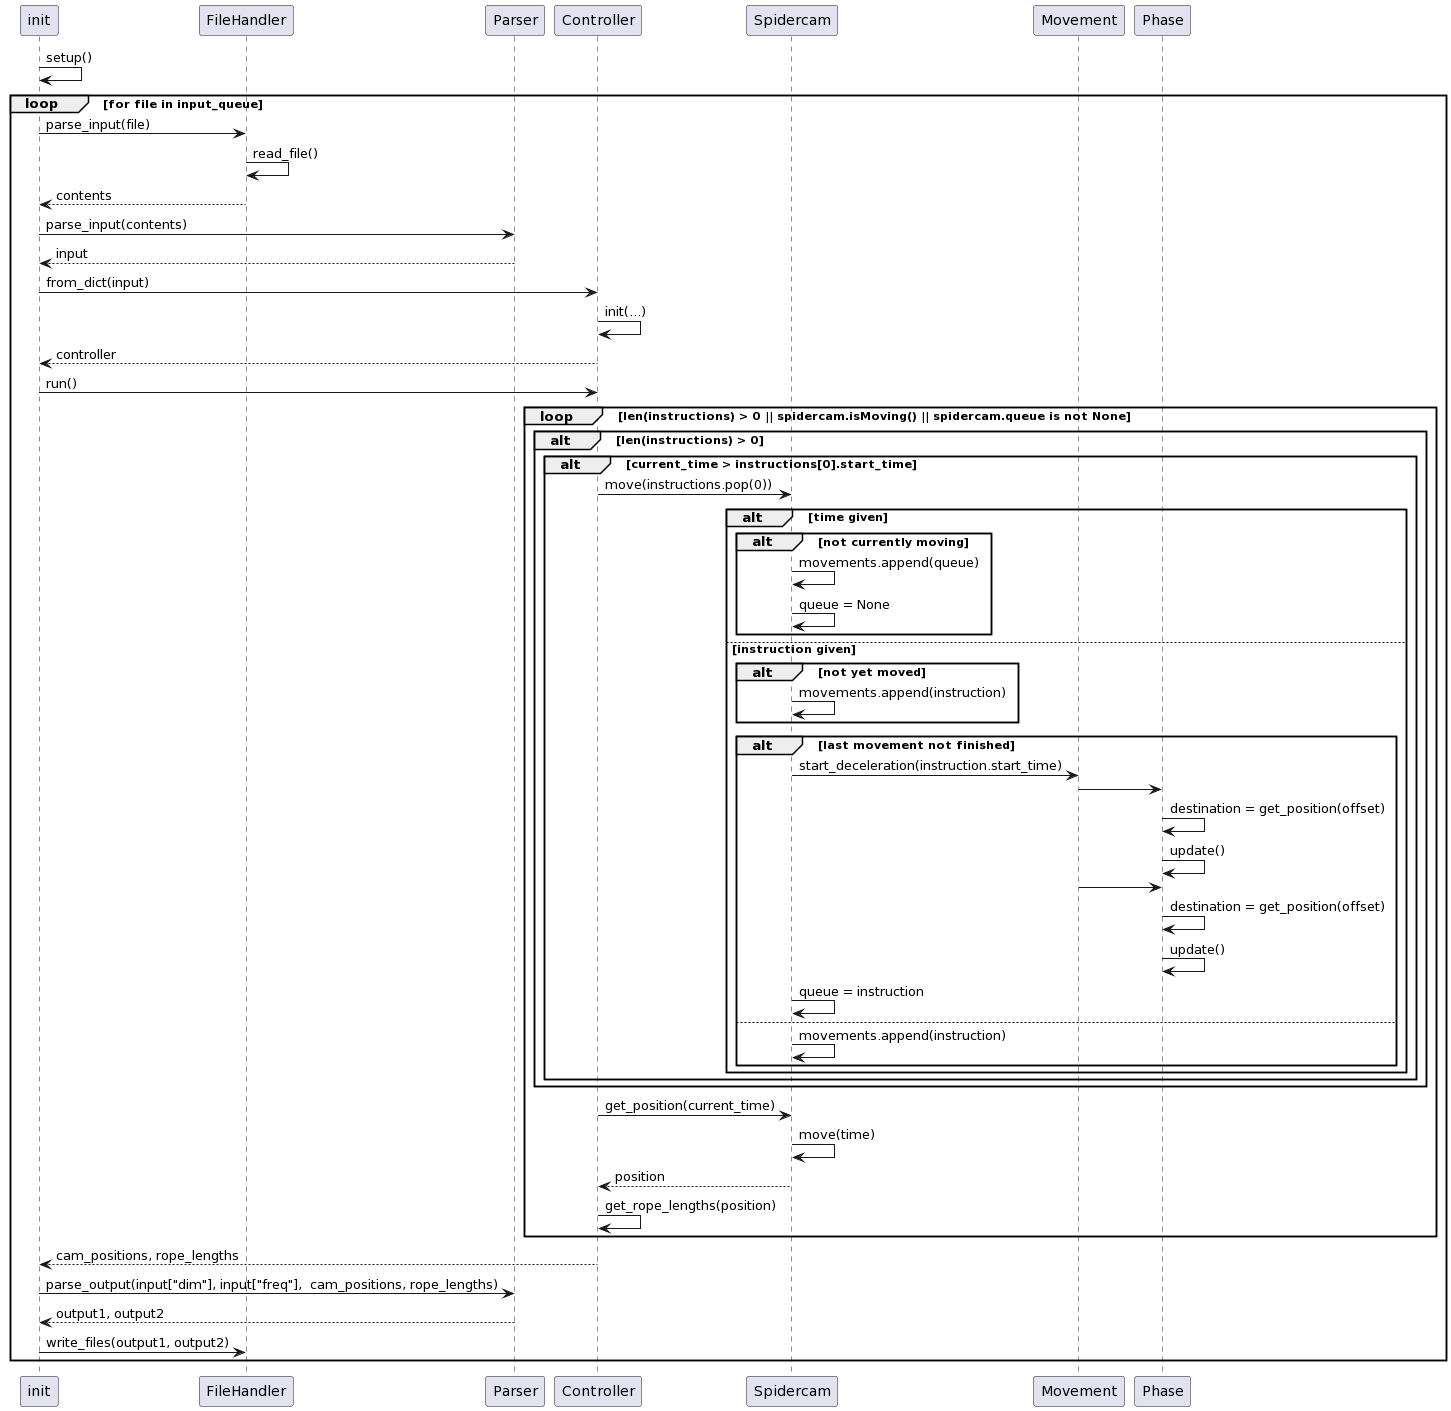
\includegraphics[width=\textwidth]{../python/uml/sequence.png}
    \caption{Aufrufhierarchie des Programms}
    \label{fig:sequence}
\end{figure}

\subsection{Beispielablauf}
\label{sssec:beispielablauf}

% Beschreibung des Beispielablaufs
Gegeben sei der Input der Datei \texttt{IHK\_2.txt}, siehe \ref{sec:testdateien}.

\begin{itemize}
    \item In der \texttt{\_\_main\_\_.py} wird mithilfe der Klassen \texttt{FileHandler} und \texttt{Parser} die Datei eingelesen und damit eine \texttt{Controller}-Instanz erzeugt, die wiederum ebenfalls eine \texttt{Spidercam}-Instanz erzeugt.
    \item Mithilfe der Funktion \texttt{run()} wird nun der Kern des Programmablaufs gestartet.
    \item Die Spidercam befindet sich zum Start an den Koordinaten $s = (10, 80, 10)$.
    \item Die Maximalgeschwindigkeit der Spidercam ist $v_{\max} = 6$ mit einer Beschleunigung von $a = 2$.
    \item Die Zeit wird auf $0$ gesetzt und von nun an in $0.5$-Sekunden-Schritten erhöht.

    \item Für den Zeitpunkt $0$ existiert eine Instruktion mit Zielkoordinaten $k_1 = (50, 40, 30)^T$.
    \item Der \texttt{Controller} weist mit \texttt{move(instruction)} die Spidercam an, sich zu diesen Koordinaten zu bewegen.
    \item Sie überprüft, ob die bisherige Bewegung abgeschlossen ist. Dies ist der Fall, da bisher noch keine Bewegung stattgefunden hat.
    \item Die leere Liste der Bewegungen \texttt{movements} wird nun mit einer neuen Instanz der Klasse \texttt{Movement} erweitert, initialisiert mit den Startkoordinaten der Spidercam und den Zielkoordinaten der Instruktion.
          \begin{itemize}
              \item Anhand der Distanz $d(s, k_1)$ wird bestimmt, wie viele Phasen die Bewegung benötigt.
              \item Es gilt $d(s, k_1) = \|(k_1 - s)\| = 60$.
              \item Da $d(s, k_1) > 2 \cdot v_{\max} \cdot a^{-1}$, wird die Bewegung in drei Phasen unterteilt.
              \item Die erste Phase ist eine Beschleunigungsphase mit Start $s$ und Ziel
                    \[ p_1 = s + \frac{v_{\max} \cdot a^{-1}}{d(s, k_1)} \cdot (k_1 - s) = (16, 74, 13)^T \]
              \item Die zweite Phase ist eine Konstantgeschwindigkeitsphase mit Start $p_1$ und Ziel
                    \[ p_2 = k_1 - \frac{v_{\max} \cdot a^{-1}}{d(s, k_1)} \cdot (k_1 - s) = (44, 46, 27)^T \]
              \item Die dritte Phase ist eine Bremsphase mit Start $p_2$ und Ziel $k_1$.
              \item Die Phasen werden nun in die Bewegung eingefügt.
          \end{itemize}
    \item Für alle Zeitpunkte bis zur nächsten Instruktion beim Zeitpunkt 20 werden nun die Position der Spidercam berechnet.
          \begin{itemize}
              \item Der \texttt{Controller} ruft mit die Funktion \texttt{get\_position(time)} der Spidercam auf.
              \item Die Spidercam bestimmt, ob der Zeitpunkt in, zwischen, vor oder nach einer Bewegung liegt.
              \item Die Fälle zwischen, vor und nach sind trivial, da die Spidercam in diesen Fällen einfach die Start- bzw. Endposition der Bewegung zurückgibt.
              \item Wird das \texttt{Movement} gefunden, in dem sich der Zeitpunkt befindet, bestimmt dieses die Position der Spidercam.
                    \begin{itemize}
                        \item Es wird bestimmt, in welcher Phase sich der Zeitpunkt befindet und welcher Offset $t_o$ innerhalb der Phase erreicht wurde.
                        \item Entsprechend der Phase, der Startgeschwindigkeit $v_s$ und des Offsets kann die Position der Spidercam berechnet werden:
                              \[
                                  s(t_o) = \begin{cases}
                                      \frac{a\cdot t_o^2}{2}                   & \text{für die Beschleunigungsphase}          \\
                                      v_{\max} \cdot t                         & \text{für die Konstantgeschwindigkeitsphase} \\
                                      v_{s} \cdot t_o - \frac{a\cdot t_o^2}{2} & \text{für die Bremsphase}
                                  \end{cases}
                              \]
                        \item Die Position entspricht dann der Startposition der Bewegung plus der entsprechend skalierten Richtung.
                    \end{itemize}
              \item Mithilfe der Position der Spidercam werden nun auch die Längen der Drahtseile bestimmt und gespeichert.
          \end{itemize}
    \item Für den Zeitpunkt 20 existiert eine Instruktion mit Zielkoordinaten $k_2 = (10, 80, 10)^T$.
    \item Die Spidercam hat ihre bisherige Bewegung abgeschlossen.
    \item \texttt{movements} wird nun analog zu vorher mit einer neuen \texttt{Movement}-Instanz erweitert.
    \item Für die Zeitpunkte bis zur nächsten Instruktion beim Zeitpunkt 22 werden nun die Positionen der Spidercam und Längen der Seile wie oben berechnet.
    \item Zum Zeitpunkt 22 existiert eine Instruktion mit Zielkoordinaten $k_3 = (50, 40, 30)^T$.
    \item Die Spidercam hat ihre bisherige Bewegung noch nicht abgeschlossen.
    \item Die Spidercam ruft die Funktion \texttt{start\_deceleration(time)} auf dem letzten \texttt{Movement} auf.
          \begin{itemize}
              \item Es wird die Phase der Bewegung bestimmt, in der sich der Zeitpunkt befindet.
              \item Der Endpunkt dieser Phase wird auf den aktuellen Zeitpunkt gesetzt und die Phase geupdated.
              \item Die folgende Phase wird zu einer Bremsphase abgeändert und das Ziel entsprechend \ref{ssec:mathematische_modellierung} bestimmt.
          \end{itemize}
    \item Mithilfe der aktualisierten Bewegung wird nun ein neues \texttt{Movement} erzeugt mit dem Ende der letzten Bewegung als Start ($s' = (44.66, 45.33, 27.33)^T$) und Ziel $k_3$.
    \item Die Entfernung der beiden Koordinaten ist kleiner als $2 \cdot v_{\max} \cdot a^{-1}$, sodass die Bewegung zweiphasig ist.
          \begin{itemize}
              \item Die erste Phase ist eine Beschleunigungsphase mit Start $s$ und Ziel
                    \[ p_1 = s + \frac{d(s', k_3)}{2} \cdot (k_3 - s') = (47.33, 45.33, 27.33)^T \]
              \item Die zweite Phase ist eine Konstantgeschwindigkeitsphase mit Start $p_1$ und Ziel $k_3$.
          \end{itemize}
    \item Dieses neue Objekt wird nun als \texttt{queue} der Spidercam gespeichert.
    \item Erneut erfolgt die Berechnung der Positionen der Spidercam und Längen der Seile für die Zeitpunkte bis zur nächsten Instruktion beim Zeitpunkt 23.
    \item Zum Zeitpunkt 23 existiert eine Instruktion mit Zielkoordinaten $k_4 = (30, 50, 20)^T$.
    \item Die Spidercam hat ihre bisherige Bewegung noch nicht abgeschlossen, bremst allerdings schon ab. Die letzte Bewegung muss also nicht aktualisiert werden.
    \item Analog wird nun wieder ein \texttt{Movement} erzeugt und die \texttt{queue} der Spidercam überschrieben.
    \item Die Bestimmung der Zeitpunkte erfolgt wieder bis zum Zeitpunkt 27.5.
    \item Zum Zeitpunkt 27.5 existiert eine Instruktion mit Zielkoordinaten $k_5 = (10, 80, 20)^T$.
    \item Die bisherige Bewegung ist abgeschlossen, die Berechnung funktioniert also analog zur zweiten Instruktion.
    \item Nach Abschluss dieser letzten Instruktion terminiert die \texttt{run()}-Funktion des \texttt{Controller}s.
    \item Die Funktion gibt die Liste der berechneten Kamerapositionen und Längen der Drahtseile zurück, die dann entsprechend in Ausgabedateien geschrieben werden.
\end{itemize}
